\section{Aim}
 To study the basic PLpg/SQL and SEQUENCE queries.

\section{{Theory}}

PL/pgSQL is a loadable procedural language for the PostgreSQL database system. The design goals of PL/pgSQL were to create a loadable procedural language that

\begin{itemize}
    \item can be used to create functions and trigger procedures,
    \item adds control structures to the SQL language,
    \item can perform complex computations,
    \item inherits all user-defined types, functions, and operators,
    \item can be defined to be trusted by the server,
\end{itemize}

SQL, the query language used by most relational database models, requires that the server runs each query individually. This means that the application must send each query to the database server, wait for it to be processes, recieve and process the results, then send further queries to the server. 

With PLpg/SQL, you can group a set of queries in the server, and then execute the group at once, hence reducing the time required. 

\section{{Code and Output}}

\begin{enumerate}
\item To print the first ‘n’ prime numbers.\newline
\begin{minted}{sql}
CREATE OR REPLACE FUNCTION primes(n INTEGER)
RETURNS INTEGER AS
$$
DECLARE
counter INTEGER := 0;
i INTEGER := 2;
prime_list TEXT;
divisors INTEGER := 0;
BEGIN
WHILE counter < n LOOP
FOR j IN 2..i/2 LOOP
IF (i%j = 0) THEN
divisors := divisors + 1;
END IF;
END LOOP;
IF (divisors = 0) THEN
RAISE NOTICE '%', i;
counter := counter + 1;
END IF;
divisors := 0;
i := i + 1;
END LOOP;
RETURN NULL;
END;
$$ LANGUAGE plpgsql;
\end{minted}
\newline
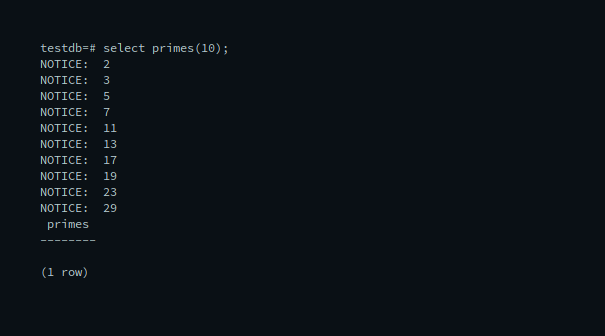
\includegraphics[width=\linewidth]{../Images/Plsql/1.png}

\item Display the Fibonacci series upto ‘n’ terms.\newline
\begin{minted}{sql}
CREATE OR REPLACE FUNCTION fibonacci (n INTEGER)
RETURNS INTEGER AS $$
DECLARE
i INTEGER := 0 ;
j INTEGER := 1 ;
BEGIN

IF (n < 1) THEN
RETURN null ;
END IF;

LOOP
EXIT WHEN i > n ;
raise notice '%', i;
SELECT j, i + j INTO i,   j ;
END LOOP ;

RETURN null;
END ;
$$ LANGUAGE plpgsql;
\end{minted}
\newline
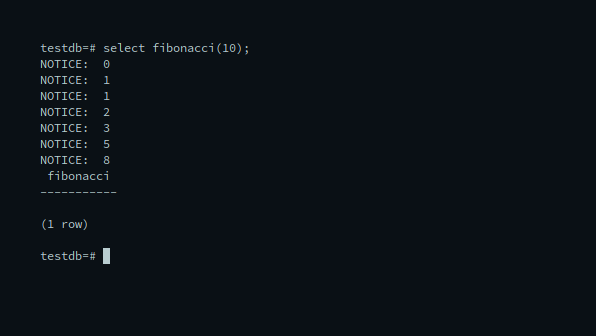
\includegraphics[width=\linewidth]{../Images/Plsql/2.png}

\item Create a table named student\_grade with the given attributes: roll, name, mark1, mark2, mark3, grade. Calculate the grade of the student and insert a it into the table using PL/SQL. ( Grade= 'PASS' if AVG greater than 40, Grade ='FAIL' otherwise.)\newline
\begin{minted}{sql}
CREATE OR REPLACE FUNCTION marks()
RETURNS INTEGER
AS $$
DECLARE
total INTEGER := 0;
BEGIN
UPDATE student_marks 
	SET grade='PASS' 
	WHERE (mark1 + mark2 + mark3) / 3 > 40;
UPDATE student_marks 
	SET grade='FAIL' 
	WHERE (mark1 + mark2 + mark3) / 3 <= 40;
RETURN null;
END;
$$ LANGUAGE plpgsql;
\end{minted}
\newline
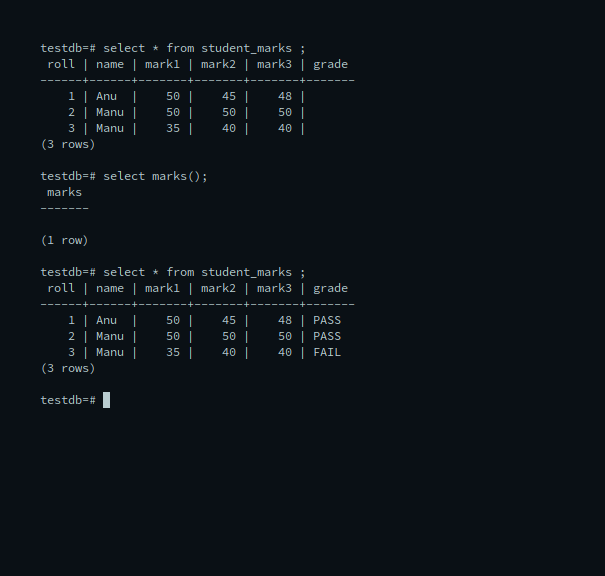
\includegraphics[width=\linewidth]{../Images/Plsql/3.png}

\item Create table circle\_area (rad,area). For radius 5, 10, 15, 20 and 25, find the area and insert the corresponding values into the table by using loop structure in PL/SQL.\newline
\begin{minted}{sql}
CREATE OR REPLACE FUNCTION area()
RETURNS TABLE(r REAL, area REAL)
AS $$
BEGIN

FOR r IN 1..5 LOOP
INSERT INTO circles VALUES(5*r, 22*5*r/7);
END LOOP;
RETURN QUERY SELECT * FROM circles;
END;
$$ LANGUAGE plpgsql;
\end{minted}
\newline
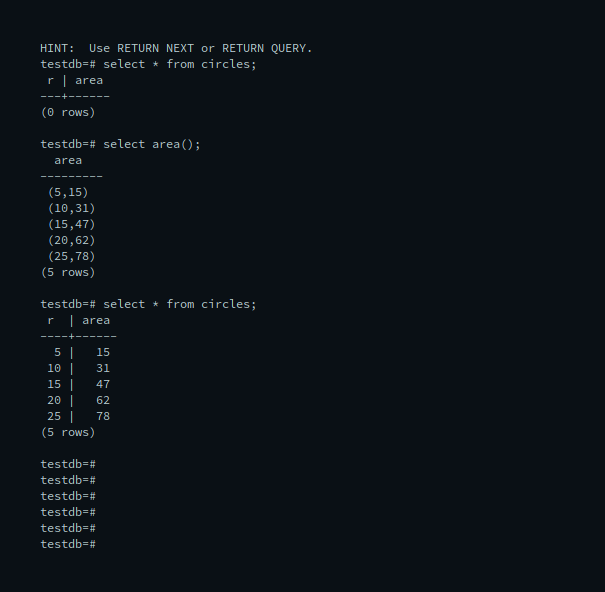
\includegraphics[width=\linewidth]{../Images/Plsql/4.png}

\item Use an array to store the names and marks of 10 students in a class. Using loop structures in PL/SQL insert the ten tuples to a table named stud. \newline
\begin{minted}{sql}
CREATE OR REPLACE FUNCTION students_data_entry()
RETURNS INTEGER
AS $$
DECLARE
names TEXT ARRAY := '{
	"ARUN",
	"AMAL",
	"PETER",
	"JOSE",
	"ANNIE",
	"MARY",
	"JOSEPH",
	"MARK",
	"MIDHUN",
	"KEVIN"}';
marks INTEGER ARRAY := '{
	25,
	76,
	43,
	45,
	67,
	57,
	97,
	56,
	89,
	8}';
BEGIN
FOR i IN 1..10 LOOP
INSERT INTO students_data VALUES (names[i], marks[i]);
END LOOP;
RETURN null;
END;
$$ LANGUAGE plpgsql;
\end{minted}
\newline
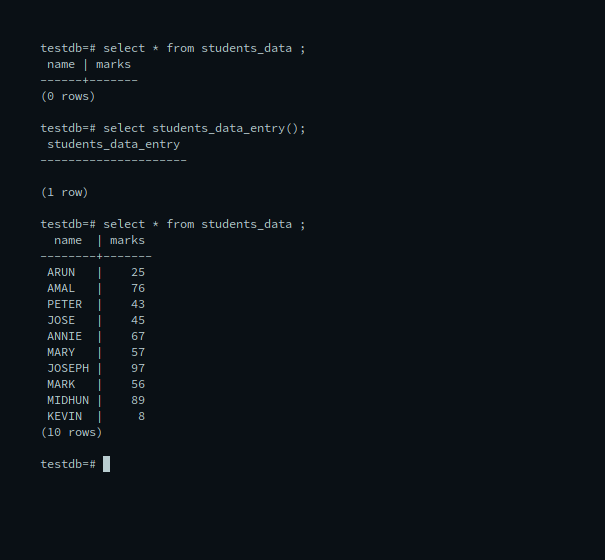
\includegraphics[width=\linewidth]{../Images/Plsql/5.png}

\item Create a sequence using PL/SQL. Use this sequence to generate the primary key values for a table named class\_cse with attributes roll, name and phone\_no. Insert some tuples using PL/SQL programming.\newline
\begin{minted}{sql}
CREATE OR REPLACE FUNCTION generate_data()
RETURNS INTEGER
AS $$
BEGIN
CREATE SEQUENCE numbers;
INSERT INTO class_cse 
	VALUES(nextval('numbers'), 'ARUN', '0482-239091');
INSERT INTO class_cse 
	VALUES(nextval('numbers'), 'AMAL', '0484-234562');
INSERT INTO class_cse 
	VALUES(nextval('numbers'), 'PETER', '0485-11234');
INSERT INTO class_cse 
	VALUES(nextval('numbers'), 'JOSE', '0481-43617');
DROP SEQUENCE numbers;
RETURN null;
END;
$$ LANGUAGE plpgsql;
\end{minted}
\newline
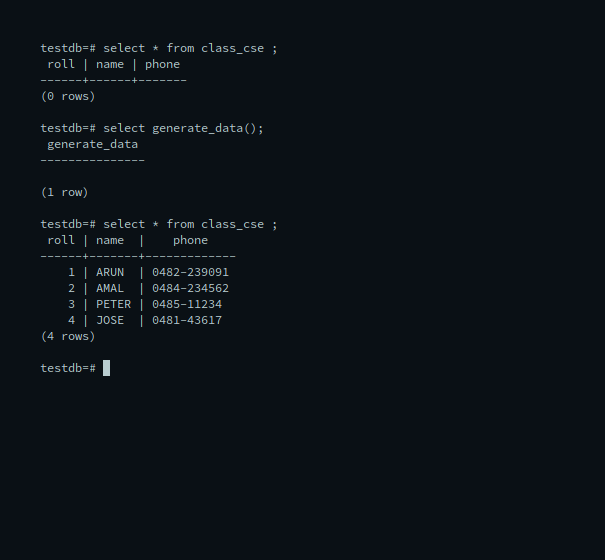
\includegraphics[width=\linewidth]{../Images/Plsql/6.png}

\end{enumerate}

\section{Result}
Implemented the program for PL/SQL and Sequence using Postgresql 11.5 on Manjaro Linux and the output was obtained.